% Options for packages loaded elsewhere
\PassOptionsToPackage{unicode}{hyperref}
\PassOptionsToPackage{hyphens}{url}
%
\documentclass[
  12pt,
]{article}
\usepackage{amsmath,amssymb}
\usepackage{lmodern}
\usepackage{iftex}
\ifPDFTeX
  \usepackage[T1]{fontenc}
  \usepackage[utf8]{inputenc}
  \usepackage{textcomp} % provide euro and other symbols
\else % if luatex or xetex
  \usepackage{unicode-math}
  \defaultfontfeatures{Scale=MatchLowercase}
  \defaultfontfeatures[\rmfamily]{Ligatures=TeX,Scale=1}
\fi
% Use upquote if available, for straight quotes in verbatim environments
\IfFileExists{upquote.sty}{\usepackage{upquote}}{}
\IfFileExists{microtype.sty}{% use microtype if available
  \usepackage[]{microtype}
  \UseMicrotypeSet[protrusion]{basicmath} % disable protrusion for tt fonts
}{}
\makeatletter
\@ifundefined{KOMAClassName}{% if non-KOMA class
  \IfFileExists{parskip.sty}{%
    \usepackage{parskip}
  }{% else
    \setlength{\parindent}{0pt}
    \setlength{\parskip}{6pt plus 2pt minus 1pt}}
}{% if KOMA class
  \KOMAoptions{parskip=half}}
\makeatother
\usepackage{xcolor}
\usepackage[margin=1in]{geometry}
\usepackage{color}
\usepackage{fancyvrb}
\newcommand{\VerbBar}{|}
\newcommand{\VERB}{\Verb[commandchars=\\\{\}]}
\DefineVerbatimEnvironment{Highlighting}{Verbatim}{commandchars=\\\{\}}
% Add ',fontsize=\small' for more characters per line
\usepackage{framed}
\definecolor{shadecolor}{RGB}{248,248,248}
\newenvironment{Shaded}{\begin{snugshade}}{\end{snugshade}}
\newcommand{\AlertTok}[1]{\textcolor[rgb]{0.94,0.16,0.16}{#1}}
\newcommand{\AnnotationTok}[1]{\textcolor[rgb]{0.56,0.35,0.01}{\textbf{\textit{#1}}}}
\newcommand{\AttributeTok}[1]{\textcolor[rgb]{0.77,0.63,0.00}{#1}}
\newcommand{\BaseNTok}[1]{\textcolor[rgb]{0.00,0.00,0.81}{#1}}
\newcommand{\BuiltInTok}[1]{#1}
\newcommand{\CharTok}[1]{\textcolor[rgb]{0.31,0.60,0.02}{#1}}
\newcommand{\CommentTok}[1]{\textcolor[rgb]{0.56,0.35,0.01}{\textit{#1}}}
\newcommand{\CommentVarTok}[1]{\textcolor[rgb]{0.56,0.35,0.01}{\textbf{\textit{#1}}}}
\newcommand{\ConstantTok}[1]{\textcolor[rgb]{0.00,0.00,0.00}{#1}}
\newcommand{\ControlFlowTok}[1]{\textcolor[rgb]{0.13,0.29,0.53}{\textbf{#1}}}
\newcommand{\DataTypeTok}[1]{\textcolor[rgb]{0.13,0.29,0.53}{#1}}
\newcommand{\DecValTok}[1]{\textcolor[rgb]{0.00,0.00,0.81}{#1}}
\newcommand{\DocumentationTok}[1]{\textcolor[rgb]{0.56,0.35,0.01}{\textbf{\textit{#1}}}}
\newcommand{\ErrorTok}[1]{\textcolor[rgb]{0.64,0.00,0.00}{\textbf{#1}}}
\newcommand{\ExtensionTok}[1]{#1}
\newcommand{\FloatTok}[1]{\textcolor[rgb]{0.00,0.00,0.81}{#1}}
\newcommand{\FunctionTok}[1]{\textcolor[rgb]{0.00,0.00,0.00}{#1}}
\newcommand{\ImportTok}[1]{#1}
\newcommand{\InformationTok}[1]{\textcolor[rgb]{0.56,0.35,0.01}{\textbf{\textit{#1}}}}
\newcommand{\KeywordTok}[1]{\textcolor[rgb]{0.13,0.29,0.53}{\textbf{#1}}}
\newcommand{\NormalTok}[1]{#1}
\newcommand{\OperatorTok}[1]{\textcolor[rgb]{0.81,0.36,0.00}{\textbf{#1}}}
\newcommand{\OtherTok}[1]{\textcolor[rgb]{0.56,0.35,0.01}{#1}}
\newcommand{\PreprocessorTok}[1]{\textcolor[rgb]{0.56,0.35,0.01}{\textit{#1}}}
\newcommand{\RegionMarkerTok}[1]{#1}
\newcommand{\SpecialCharTok}[1]{\textcolor[rgb]{0.00,0.00,0.00}{#1}}
\newcommand{\SpecialStringTok}[1]{\textcolor[rgb]{0.31,0.60,0.02}{#1}}
\newcommand{\StringTok}[1]{\textcolor[rgb]{0.31,0.60,0.02}{#1}}
\newcommand{\VariableTok}[1]{\textcolor[rgb]{0.00,0.00,0.00}{#1}}
\newcommand{\VerbatimStringTok}[1]{\textcolor[rgb]{0.31,0.60,0.02}{#1}}
\newcommand{\WarningTok}[1]{\textcolor[rgb]{0.56,0.35,0.01}{\textbf{\textit{#1}}}}
\usepackage{graphicx}
\makeatletter
\def\maxwidth{\ifdim\Gin@nat@width>\linewidth\linewidth\else\Gin@nat@width\fi}
\def\maxheight{\ifdim\Gin@nat@height>\textheight\textheight\else\Gin@nat@height\fi}
\makeatother
% Scale images if necessary, so that they will not overflow the page
% margins by default, and it is still possible to overwrite the defaults
% using explicit options in \includegraphics[width, height, ...]{}
\setkeys{Gin}{width=\maxwidth,height=\maxheight,keepaspectratio}
% Set default figure placement to htbp
\makeatletter
\def\fps@figure{htbp}
\makeatother
\setlength{\emergencystretch}{3em} % prevent overfull lines
\providecommand{\tightlist}{%
  \setlength{\itemsep}{0pt}\setlength{\parskip}{0pt}}
\setcounter{secnumdepth}{-\maxdimen} % remove section numbering
\usepackage{setspace}\doublespacing
\usepackage{amsmath}
\usepackage{lineno}
\linenumbers
\usepackage{fontspec}
\setmainfont{Times New Roman}
\usepackage{placeins}
\usepackage{booktabs}
\usepackage{longtable}
\usepackage{array}
\usepackage{multirow}
\usepackage{wrapfig}
\usepackage{float}
\usepackage{colortbl}
\usepackage{pdflscape}
\usepackage{tabu}
\usepackage{threeparttable}
\usepackage{threeparttablex}
\usepackage[normalem]{ulem}
\usepackage{makecell}
\usepackage{xcolor}
\ifLuaTeX
  \usepackage{selnolig}  % disable illegal ligatures
\fi
\IfFileExists{bookmark.sty}{\usepackage{bookmark}}{\usepackage{hyperref}}
\IfFileExists{xurl.sty}{\usepackage{xurl}}{} % add URL line breaks if available
\urlstyle{same} % disable monospaced font for URLs
\hypersetup{
  pdftitle={Bayesian hierarchical modeling of size spectra},
  hidelinks,
  pdfcreator={LaTeX via pandoc}}

\title{Bayesian hierarchical modeling of size spectra}
\author{}
\date{\vspace{-2.5em}}

\begin{document}
\maketitle

Jeff S. Wesner, Justin P.F. Pomeranz, James R. Junker, Vosjava Gjoni,
Yuhlong Lio

University of South Dakota, Department of Biology, Vermillion, SD 5706

Colorado Mesa University

Louisiana University Marine Consortium

Michigan State University

University of South Dakota, Department of Mathematics, Vermillion, SD
57069

\href{mailto:Jeff.Wesner@usd.edu}{\nolinkurl{Jeff.Wesner@usd.edu}}

\newpage

\textbf{Abstract}

A fundamental pattern in ecology is that smaller organisms are more
abundant than larger organisms. At the individual level, this pattern is
known as the individual size distribution (ISD) or community size
spectrum, which describes the frequency distribution of all individuals
in an ecosystem, regardless of taxon. This distribution arises from a
power law distribution, such as the Pareto distribution, and a major
goal of size spectra analyses is to estimate the ISD power law exponent.
However, while numerous methods have been developed, they have focused
almost exclusively on estimating the exponent from single samples. Here,
we develop an extension of the truncated Pareto distribution within the
probabilistic modeling language Stan. We use it to estimate multiple ISD
exponents simultaneously with a hierarchical modeling approach. The most
important result is the ability to examine hypotheses related to size
spectra within a single generalized (non)-linear mixed model.

Keywords: \emph{Bayesian, body size spectra, hierarchical, Pareto, power
law, Stan}

\newpage

\textbf{Introduction}

In any ecosystem, large individuals are typically more rare than small
individuals. This fundamental feature of ecosystems generates a
remarkably common pattern in which relative abundance declines with
individual body size, generating the individual size distribution ISD
(or community size spectrum) (Sprules and Barth 1983; White et
al.~2008). More formally, the ISD is a frequency distribution that can
be approximated by a bounded power law with a single free parameter
\(\lambda\), corresponding to the following probability density function
(Edwards et al.~2020):

\[
f(x) = Cx^\lambda, x_{min} \le x \ge x_{max}
\]

where \(x\) is the body size (e.g., mass or volume) of an individual
regardless of taxon, \(x_{min}\) is the smallest individual attainable
and \(x_{max}\) is the largest possible individual (White et al.~2008).
\(C\) is a constant equal to:

\[
 C = \begin{cases}\frac{\lambda + 1}{{x_{max}^{\lambda+1}} - {x_{min}^{\lambda+1}}}, \lambda \neq-1 \\
\frac{1}{{logx_{max}^{\lambda+1}} - {logx_{min}^{\lambda+1}}}, \lambda = -1\end{cases}
\]

This model is also known as the bounded power law or truncated Pareto
distribution. The terms ``bounded'' or ``truncated'' refer to the limits
of \(x_{min}\) and \(x_{max}\). Without those limits, the function is a
simple power law. Each term in the equations above comes directly from
the data except for the exponent \(\lambda\), which must be estimated
from a statistical model.

The exponent \(\lambda\) is often described by its ``steepness'', with
more negative values (i.e., ``steeper'') indicating higher abundance of
large relative to small individuals, and vice versa. These patterns of
size frequency are an emergent property of demographic processes (e.g.,
age-dependent mortality), ecological interactions (e.g., size-structured
predation, trophic transfer efficiency), and physiological constraints
(e.g., size-dependent metabolic rates) (Andersen and Beyer 2006, White
et al.~2008). As a result, variation in \(\lambda\) across ecosystems or
across time can indicate fundamental shifts in community structure or
ecosystem functioning. For example, overfishing in marine communities
has been detected using size spectra in which \(\lambda\) was steeper
then expected, indicating fewer large fish than expected (Blanchard et
al.~200x). Shifts in \(\lambda\) have also been used to document
responses to acid mine drainage in streams (Pomeranz et al.~2019;
Pomeranz et al.~2020), and changes in response to land use (Martínez et
al.~2016), resource subsidies (Perkins et al.~2018), and temperature
(Pomeranz et al.~2022).

Given the ecological information it conveys, the data required to
estimate size spectra are deceptively simple; only a single column of
data are needed, in which each data point is a single measure of the
body size of an individual. As long as the body sizes are collected
systematically and without bias towards certain taxa or phenotypes,
there is no need to know any more ecological information about the data
points (e.g., taxon, trophic position, age, abundance). However, despite
the simple data requirement, the statistical models used to estimate
\(\lambda\) are diverse. Edwards et al (2017) documented 8 different
analytical methods. Six of these involved binning, in which the body
sizes are grouped into size bins (e.g., 2-49 mg, 50-150mg, etc.) and
then counted, generating values for abundance within each size bin. This
allows \(\lambda\) to be estimated using simple linear regression.
Unfortunately, the binning process also removes most of the variation in
the data, collapsing information about 1000's of individuals into just 6
or so bins. Doing so can lead to the wrong values of \(\lambda\),
sometimes drastically so (White et al.~2008, Edwards et al.~2017/2020).

An improved alternative to binning and linear regression is to fit the
body size data to a power law probability distribution (White et
al.~2008, Edwards et al.~2017/2020). This method uses all of the data
without binning and directly estimates \(\lambda\) using maximum
likelihood (Edwards et al.~2017)\emph{.} However, at present it is only
possible to fit the models to single data set using maximum likelihood.
To our knowledge there is no current method to fit ISD models to
multiple groups of ISD's, such as data collected from multiple sites or
multiple years. Instead, hypothesis testing with individual size
distributions is typically done in two steps (e.g., Pomeranz et
al.~2022). First, \(\lambda\) estimates are obtained individually from
each collection (e.g., each site or year, etc.). Then, these estimates
are used as response variables in a linear model to examine how they
relate to predictor variables (Edwards et al.~2020). A downside to this
approach is that it treats \(\lambda\) values as independent samples,
even if they come from the same sites or times. It also removes
information on sample size (number of individuals used to derive
\(\lambda\). As a result, the approach not only separates the data
generation model from the predictor variables, but it is also unable to
take advantage of partial pooling during model fitting.

Here, we develop a Bayesian model that uses the truncated Pareto
distribution to estimate \(\lambda\) in response to both fixed and
random predictor variables. The model extends the maximum likelihood
approach developed by Edwards et al.~(2020) and allows for a flexible
hierarchical structure, including partial pooling, within the modeling
language Stan (Stan Development Team 2022).

\textbf{Methods}

\emph{Translating to Stan}

We first translated the probability density function described by
Edwards et al.~(2020) into Stan by converting it to a log probability
density function (lpdf). Stan is a probabilistic modeling language that
is capable of fitting complex models, including those with custom
lpdf's. The resulting lpdf is below:

\[
 C = \begin{cases}\text{log}\frac{\lambda + 1}{{x_{max}^{\lambda+1}} - {x_{min}^{\lambda+1}}} + \lambda\text{log}x, \lambda \neq-1 \\
\text{log}({{\text{log}x_{min}} - {\text{log}x_{max}}}) + \lambda\text{log}x, \lambda = -1\end{cases}
\]

which is coded in Stan as follows:

\begin{Shaded}
\begin{Highlighting}[]

\KeywordTok{functions}\NormalTok{\{}

\DataTypeTok{real}\NormalTok{ paretocustom\_lpdf(}\DataTypeTok{real}\NormalTok{ x, }\DataTypeTok{real}\NormalTok{ b, }\DataTypeTok{real}\NormalTok{ xmin, }\DataTypeTok{real}\NormalTok{ xmax)\{}

\ControlFlowTok{if}\NormalTok{(b != {-}}\DecValTok{1}\NormalTok{)}

\ControlFlowTok{return}\NormalTok{(log((b+}\DecValTok{1}\NormalTok{) / ( xmax\textbackslash{}\^{}(b+}\DecValTok{1}\NormalTok{) {-} xmin\textbackslash{}\^{}(b+}\DecValTok{1}\NormalTok{))) + b\textbackslash{}*log(x));}

\ControlFlowTok{else}

\ControlFlowTok{return}\NormalTok{(log(log(xmin) {-} log(xmax)) + b\textbackslash{}*log(x));}
\NormalTok{  \}}

\NormalTok{\}}
\end{Highlighting}
\end{Shaded}

We call this the \(paretocustom\) distribution, which we can now use to
estimate \(\lambda\) of given a data set. For example, an intercept-only
model would look like this:

\[x_i \sim paretocustom(\lambda, x_{min}, x_{max})\]
\[\lambda = \alpha\] \[\alpha \sim Normal(\mu, \sigma)\]

where \(x_i\) is the \(i\)th individual body size, \(\lambda\) is the
size spectrum exponent, \(x_{min}\) and \(x_{max}\) are as defined
above, and \(\alpha\) is the intercept with a prior probability
distribution. In this case, we specified a Normal prior since
\(\lambda\) is continuous and can be positive or negative, but this can
be changed as needed.

The simple model above can be expanded to a generalized linear mixed
model by including fixed predictors (\(\boldsymbol\beta \textbf{X}\))
and/or varying intercepts (\(\alpha_{[x]}\)):

\[x_{ij} \sim paretocustom(\lambda_j, x_{min, j}, x_{max, j})\]
\[\lambda = \alpha + \boldsymbol\beta \textbf{X} + \alpha_{[j]} + \alpha_{[x]}\]
\[\alpha \sim Normal(\mu_{\alpha}, \sigma_{\alpha})\]
\[\beta \sim Normal(\mu_{\beta},\sigma_{\beta})\]
\[\alpha_{[j]} \sim Normal(0, \sigma_{[j]})\]
\[\sigma_{[j]} \sim Exponential(\phi)\]
\[\alpha_{[x]} \sim Normal(0, \sigma_{[x]})\]
\[\sigma_{[x]} \sim Exponential(\phi)\]

with one or more \(\beta\) regression parameters \(\boldsymbol\beta\)
for one or more fixed predictors \(\textbf{X}\), and one or more varying
intercepts \(\alpha_x\). We specify \(\alpha_{j}\) separately because it
is needed to account for the non-independence of body sizes. In other
words, each body size \(x_i\) is clustered within each site and so they
are not independent and identically distributed. The addition of a
varying intercept for each sample accounts for this non-independence. We
demonstrate how excluding the sample-specific varying intercept can lead
to overdispersion below. Prior distributions are given as \(Normal\) for
the parameters and varying intercept and \(Exponential\) for
\(\sigma{[x]}\), but these can also be changed as needed.

The model above assumes that each body size \(x\) represents a single
individual such that the data set might have many repeats for
individuals of the same size (e.g., \(x\) = \{0.2, 0.2, 0.2, 0.4, 0.4,
0.5, 9.8\}). However, when individaul body sizes are repeated in a data
set, they are often accompanied by a count or density, such that the
data set above might instead consist of two columns with \(x\) = \{0.2,
0.4, 0.5, 9.8\} and \(counts\) = \{3, 2, 1, 1\}. To analyze this more
compact data set, Edwards et al.~(2020) developed a modification of the
log probability density function to include \(counts\):

\[
 C = \begin{cases}\textit{counts}(\text{log}\frac{\lambda + 1}{{x_{max}^{\lambda+1}} - {x_{min}^{\lambda+1}}} + \lambda\text{log}x), \lambda \neq-1 \\
\textit{counts}(\text{log}({{\text{log}x_{min}} - {\text{log}x_{max}}}) + \lambda\text{log}x), \lambda = -1\end{cases}
\]

which is coded in Stan as follows:

\begin{Shaded}
\begin{Highlighting}[]

\KeywordTok{functions}\NormalTok{\{}
  \DataTypeTok{real}\NormalTok{ paretocounts\_lpdf(}\DataTypeTok{real}\NormalTok{ x, }\DataTypeTok{real}\NormalTok{ lambda, }\DataTypeTok{real}\NormalTok{ xmin, }\DataTypeTok{real}\NormalTok{ xmax, }\DataTypeTok{real}\NormalTok{ counts)\{}
    \ControlFlowTok{if}\NormalTok{(lambda != {-}}\DecValTok{1}\NormalTok{)}
    \ControlFlowTok{return}\NormalTok{(counts*(log((lambda+}\DecValTok{1}\NormalTok{) / ( xmax\^{}(lambda+}\DecValTok{1}\NormalTok{) {-} xmin\^{}(lambda+}\DecValTok{1}\NormalTok{))) + lambda*log(x)));}
    \ControlFlowTok{else}
    \ControlFlowTok{return}\NormalTok{(counts*(log(log(xmin) {-} log(xmax)) + lambda*log(x)));}
\NormalTok{  \}}
\NormalTok{\}}
\end{Highlighting}
\end{Shaded}

We refer to this as \(paretocounts\), such that the model can be fit
using:

\[x_i\sim paretocounts(\lambda, x_{min}, x_{max}, counts)\]
\[\lambda = [\text{linear or non-linear model}]\] \[\text{[priors]}\]

Aside from adding \(counts\), the model is the same as presented above.
These models (\(paretocustom\) and \(paretocounts\)) allow us to test
how the size distribution exponent, \(\lambda\), varies in response to
continuous or categorical predictors and to include hierarchical
structure as needed.

\emph{Testing the models}

The \(paretocustom\) and \(paretocounts\) lpdf's give the same results,
differing only in how the data are aggregated. For simplicity, we
demonstrate model performance here for the \(paretocounts\)
distribution, since the empirical data we used (see \emph{Case Study}
below) contains counts of individual body sizes. First, we tested for
parameter recovery using data simulated from a bounded power law with
known values of \(\lambda\). Second, we fit the model to fisheries trawl
data presented in Edwards et al.~(2020) to estimate the hypothesis that
\(\lambda\) declines over time.

\emph{Parameter recovery from simulated data}

To ensure that the models could recover known parameter values, we
simulated ten data sets from a bounded power law:

\[
x_i = (\text{u}_ix_{max}^{(\lambda+1)} +  (1-\text{u}_i)  x_{min}^{(\lambda+1)} ) ^ {\frac{(1}{(\lambda+1)}}
\]

where \(x_i\) is the individual body size from the \(i\)th simulation,
\(u_i\) is a unique draw from a \(Uniform(0,1)\) distribution, and all
other variables are the same as defined above. We set \(x_{min}\) =1 and
\(x_{max}\) = 1000, and simulated \(i\) = 1000 values from each of 10
\(\lambda\)'s ranging from -2.2 to -1.2. To generate \(counts\), we
rounded each simulated value to the nearest 0.001 and then tallied them.

We estimated the ten \(\lambda\) values in two ways. First, we fit a
separate intercept-only model to each of the ten data sets. Second, we
fit a varying intercepts model (Gelman et al.~2014). The structure of
this model is \(b = \alpha + \alpha_{[group]}\) where each group
represents and offset from the mean value of lambda.

Finally, we simulated data for a regression model with a single
continuous predictor and a varying intercept:
\(lambda = \alpha + \beta x + \alpha_{[group]}\), where \(\alpha\) =
-1.5, \(\beta\) = -0.1, and \(\sigma_{group}\) was 0.3 for n = 3 groups.
The predictor \(x\) was continuous with 3 values (-2, 0, 2) and two
replicates per value per group for n = 18 \(\lambda\)'s. After solving
for \(\lambda\) from these known parameter values, we simulated 300
individuals from each \(\lambda\) using the procedure above, with
\(x_{min}\) = 1 and \(x_{max}\) = 100. We fit this model 20 times to
measure variation in parameter recovery among model runs.

\emph{Sample Size}

We examined sensitivity to sample size (number of individual body sizes)
across three \(\lambda\) values (-2, -1.6, -1.2). For each \(\lambda\),
we varied the number of simulated individuals from 2 to 2048,
representing a \(2^n\) sequence with \(n\) ranging from 1 to 11. Each of
the 11 densities was replicated 10 times resulting in 110 datasets of
individual body sizes. We fit each data set using separate
intercept-only \(paretocounts\) models and then plotted the resulting
\(\lambda\) values as a function of sample size.

\emph{Case Studies}

To examine model performance on empirical data, we re-ran a previously
published analysis from of Edwards et al.~(2020). In Edwards' study,
size spectra exponents were first estimated separately for each sample
using maximum likelihood. Then the modeled exponents were used as
response variables in linear regression models. The goal was to test for
linear changes in size spectra over three decades using bi-yearly size
data of marine fishes collected from the International Benthic Trawl
Survey (IBTS). The data set and original model results are available in
the \texttt{sizeSpectra} package (Edwards et al.~2017). We tested the
same hypothesis as Edwards et al.~(2020), but instead of using a
two-step process we fit a single model using the \(paretocounts\) lpdf
(Eq. X).

\emph{Model Fitting}

We fit each of the above models in rstan (Stan Development Team 2022)
using 2 chains each with 1000 iterations. All models converged with
\(r_{hat}\)'s \textless1.01. If a known parameter value fell inside the
95\% Credible Intervals, we considered parameter recover successful. For
the replicated regression model, we also tallied the number of times
that the known value fell outside of the highest posterior density
interval (HPI; out 20 runs).

\emph{Data Availability Statement}

All data and code are available at
\url{https://github.com/jswesner/stan_spectra} (to be permanently
acrhived on acceptance).

\textbf{Results}

\emph{Parameter Recovery}

For models fit to simulated individual data set, all credible intervals
included the true value of \(\lambda\) and posterior medians were no
more than 0.05 units away from the true value (Table 1). Similarly, when
the same data set was fit using a varying intercepts model, the
posterior median intercept \(\alpha\) and group standard deviation
\(\sigma_{group}\) were nearly identical to the true values (Table 1).

\begin{table}

\caption{\label{tab:unnamed-chunk-1}Table X. Parameter recovery.}
\centering
\begin{tabular}[t]{l|l|r|r|r|r}
\hline
Model & Parameter & True Value & q2.5 & q50 & q97.5\\
\hline
Separate Models & λ & -2.20 & -2.22 & -2.15 & -2.09\\
\hline
Separate Models & λ & -2.09 & -2.13 & -2.06 & -2.00\\
\hline
Separate Models & λ & -1.98 & -2.05 & -1.99 & -1.92\\
\hline
Separate Models & λ & -1.87 & -1.91 & -1.85 & -1.80\\
\hline
Separate Models & λ & -1.76 & -1.83 & -1.78 & -1.72\\
\hline
Separate Models & λ & -1.64 & -1.70 & -1.66 & -1.61\\
\hline
Separate Models & λ & -1.53 & -1.59 & -1.54 & -1.50\\
\hline
Separate Models & λ & -1.42 & -1.48 & -1.44 & -1.40\\
\hline
Separate Models & λ & -1.31 & -1.31 & -1.28 & -1.24\\
\hline
Separate Models & λ & -1.20 & -1.26 & -1.23 & -1.20\\
\hline
Single Model with Varying Intercepts & α & -1.70 & -1.96 & -1.71 & -1.50\\
\hline
Single Model with Varying Intercepts & σ\_[group] & 0.34 & 0.23 & 0.36 & 0.58\\
\hline
\end{tabular}
\end{table}

Using the varying intercept model to estimate group specific means
yielded similar results as using separate models per group (Figure 1),
demonstrating that a single model can be used to estimate multiple size
spectra simultaneously.

\begin{figure}
\centering
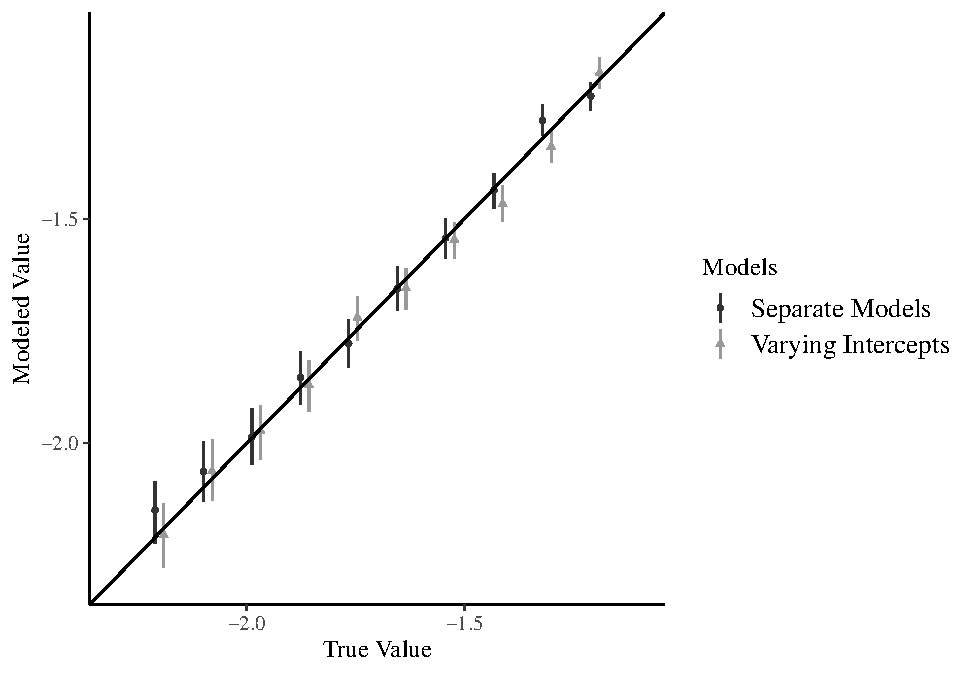
\includegraphics{stan_spectra_manuscript_update_files/figure-latex/unnamed-chunk-2-1.pdf}
\caption{Modeled estimates (median +/- 95\% Credible Intervals of λ
using either 10 separate models or a single model with ten varying
intercepts.}
\end{figure}

We also recovered regression parameters (intercept \(\alpha\) and slope
\(\beta\)) along with the group-level sd (\(\sigma_{group}\)) (Figure
2). Fitting this model 20 times indicated reliable fit. For example, out
of 60 comparison (3 parameters x 20 replicates) the true value fell
outside of the 95\% HDI only once (Figure 2). Averaging the deviations
(posterior median minus the true value) among the replicates indicated
no bias in the modeled estimates (mean bias +/- sd: \(\alpha\) = 0 +/-
0.05, \(\beta\) = 0 +/- 0.008, \(\sigma_{group}\) = 0.03 +/- 0.06).

\begin{figure}
\centering
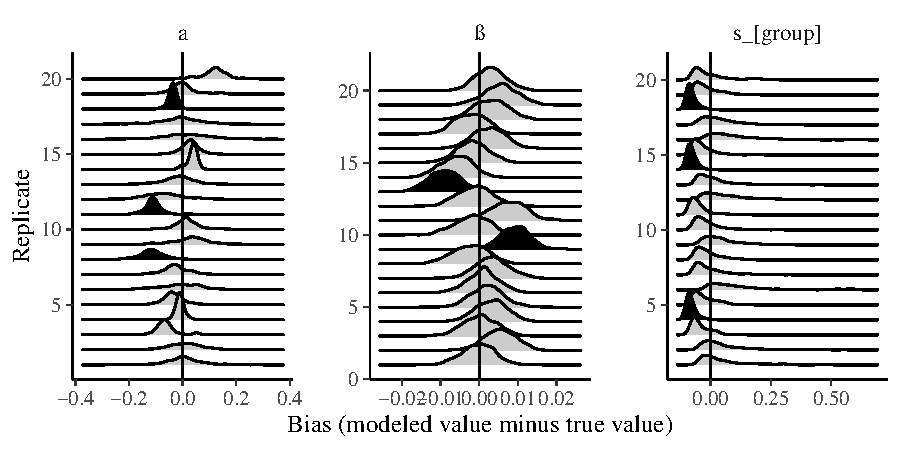
\includegraphics{stan_spectra_manuscript_update_files/figure-latex/unnamed-chunk-3-1.pdf}
\caption{Posterior distributions of n = 20 modeled estimates of alpha,
beta, and sigma\_group for a linear regression estimating the size
sepctrum exponent as a function of a continuous predictor. All data were
simulated. Gray densities indicate that the HPI contains the true value,
while black densities indicat the opposite. The vertical lines indicate
true values.}
\end{figure}

\emph{Sample Size}

Variation in modeled estimates was high for samples containing less than
100 individual (Figure 2). For example, when the true \(\lambda\) value
was -2, samples with just 8 individuals yielded estimates ranging from
-2.7 to -1.7. By contrast, all samples with more than 300 individuals
captured the true \(\lambda\) with less than 0.1 unit of error (Figure
3).

\begin{figure}
\centering
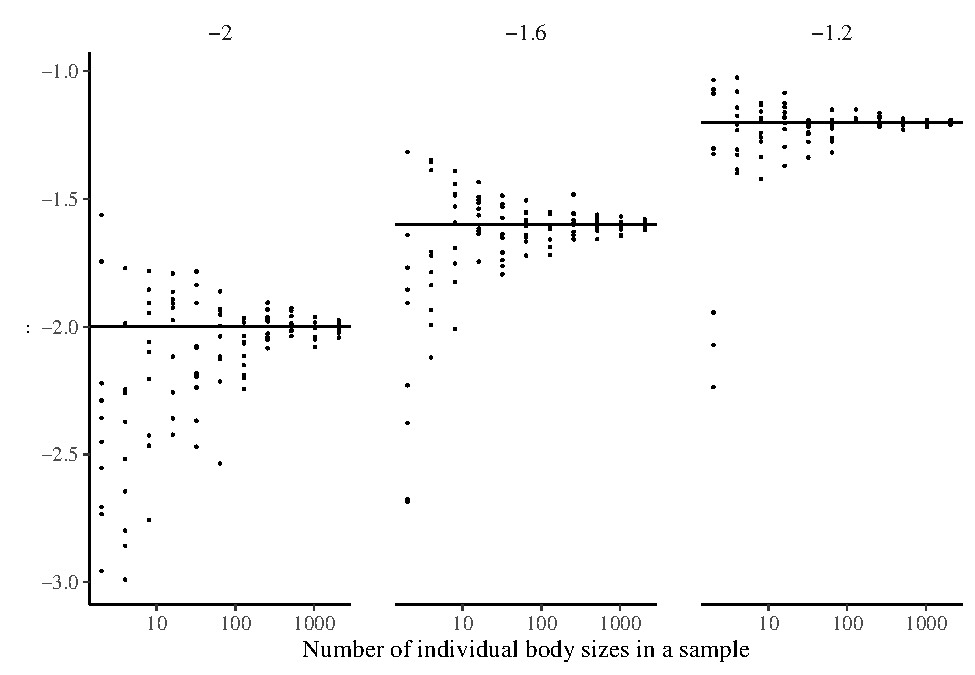
\includegraphics{stan_spectra_manuscript_update_files/figure-latex/unnamed-chunk-4-1.pdf}
\caption{Estimates of λ across 11 different sample sizes (ranging from 2
to 2048 individuals) and three different true λ's (-2, -1.6, -1.2). Ten
separate models were fit for each of the 11 sample sizes. The horizontal
lines show the true value of λ}
\end{figure}

\emph{Case Study}

Using IBTS data with the Bayesian hierarchical regression, we found a
negative trend over time. The ISD exponent of IBTS trawl data declined
by \textasciitilde0.001 units per year, but with a 95\% CrI ranging from
-0.005 to 0.002. These values were nearly identical to those reported by
Edwards et al.~(2020) using a two-step approach (Table 3).

\begin{table}

\caption{\label{tab:unnamed-chunk-5}Table X. Slope values from a regression testing the relationship between the ISD exponent and year for IBTS trawl data (Edwards et al. 2020). The values are derived using the Bayesian hierarchical model presentd here or from the maximum likelihood approach described in Edwards et al. 2020).}
\centering
\begin{tabular}[t]{l|r|r|r}
\hline
Model & Mean & q2.5 & q97.5\\
\hline
Bayesian - one step & -0.001 & -0.005 & 0.002\\
\hline
MLE - two steps & -0.001 & -0.005 & 0.003\\
\hline
\end{tabular}
\end{table}

An advantage of fitting the model in a single Bayesian hierarchical
framework is that estimates for individual groups are pulled toward the
mean via partial pooling. This is apparent in comparing the unpooled MLE
estimates (Figure Xa) to the partially pooled Bayesian estimates in each
year (Figure Xb).

\begin{figure}
\centering
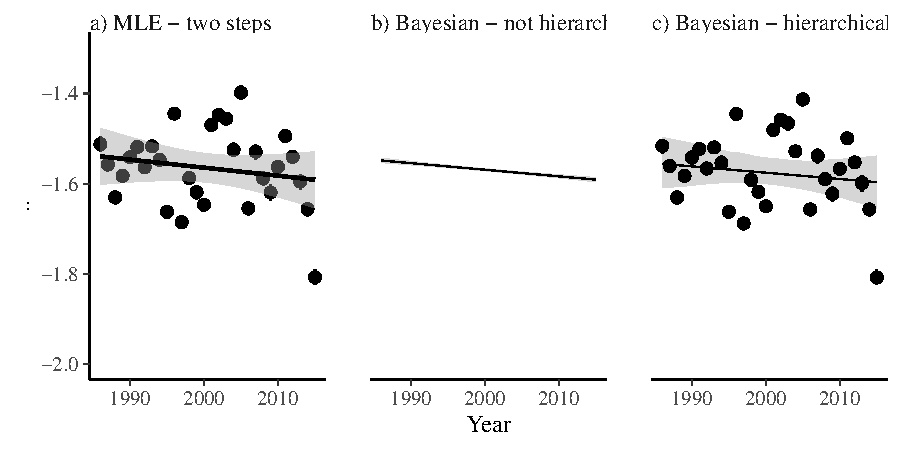
\includegraphics{stan_spectra_manuscript_update_files/figure-latex/unnamed-chunk-6-1.pdf}
\caption{Regression results from a) Edwards et al.~(2020) using maximum
likelihood and linear regression (two steps), b) the Bayesian model with
a paretocounts lpdf (one step), but without varying intercepts, and c)
the Bayesian model with varying intercepts. In a) the points represent
maximume likelihood estimates calculated separately for each year. In c)
they represent hierarchical varying intercepts calculated from the
model. There are no points in (b) because the model does not estimate
lambda for individual years.}
\end{figure}

\textbf{Discussion}

The most important result of this work is the ability to analyze ISD
exponents using fixed and random predictors in a hierarchical model. Our
approach allows ecologists to test hypotheses about size spectra while
avoiding the pitfalls of binning, which loses information and can lead
to biased estimates of \(\lambda\) (White et al.~2008). Maximum
likelihood solves this problem by directly estimating the ISD, but
testing hypotheses with maximum likelihood still requires a two-step
process in which \(\lambda\) is estimated individually for each sample
and the results are then used as response variables in linear or
non-linear models (Edwards et al.~2020). Our approach merges these
steps, allowing for the incorporation of prior probabilities and
hierarchical structure.

The ability to incorporate prior information using Bayesian updating has
two practical advantages over analysis with maximum likelihood. First,
adding informative prior distributions can improve model fit by limiting
the MCMC sampler to reasonable sampling space. In other words it would
not be sensible to estimate the probability that \(\lambda\) is -1,234
or -9. Without informative priors, those values (and more extreme
values) are considered equally likely and hence waste much of the
algorithms sampling effort on unlikely values (e.g., Wesner et
al.~2021).

Second, and most importantly, ecologists have much prior information on
the values that \(\lambda\) can take. For example, Sheldon's conjecture
suggests that \(\lambda\) is -2.05 (Andersen et al.~2006), a value
supported in pelagic marine ecosystems (Glazier et al.~XXXX) and among
forest trees (Enquist et al.~I THINK?). However, benthic marine systems
typically have shallower exponents (e.g., \textasciitilde-1.4; Blanchard
et al.~200X), while freshwater stream ecosystems have values somewhere
in between (-1.5; Pomeranz et al.~2022). However, despite apparent
variation among ecocystems, there is a strong indication that the values
of \(\lambda\) are most likely to be somewhere between -2.05 and -1.4
for many ecosystems. As a result, a prior that places most of its
probability mass on these values (e.g., \(Normal(-1.6, 0.2)\) seems
appropriate. Such a continuous prior does not prevent findings of larger
or smaller \(\lambda\), but instead places properly weighted skepticism
on such values.

Similar to priors, partial pooling from varying intercepts provides
additional benefits, allowing for the incorporation of hierarchical
structure and pulling \(\lambda\) estimates towards the global mean
(Gelman et al.~2005, Qian et al.~2010). In the examples shown here, the
amount of pooling is relatively small because the sample sizes are large
(\textgreater1000 individuals). However, the primary benefits of pooling
(both from varying effects and skeptical priors) is in prediction
(Gelman et al.~2005, Hobbs and Hooten 2015). This becomes especially
important when models are used to forecast future ecosystem conditions.
We are unaware of efforts to forecast ISD's, but such forecasts seem to
be especially useful with modern long-term data sets like NEON (National
Ecological Observatory Network) in which body size samples will be
collected at the continental scale over at least the next 20 years
(Loescher et al.~2016). In addition, because the effects of priors and
pooling increase with smaller samples sizes, varying intercepts are
likely to be particularly helpful for small samples. In other words,
priors and partial pooling contain built-in skepticism of extreme
values, ensuring the maxim that ``extraordinary claims require
extraordinary evidence''.

One major drawback to the Bayesian modeling framework here is time.
Bayesian models of even minimal complexity must be estimated with Markov
Chain Monte Carlo techniques. In this study, we used the Hamiltonion
Monte Carlo (HMC) algorithm with a No-U-Turn Sampler (NUTS) via
\texttt{rstan} (Stan Development Team 2022). Stan is substantially
faster than other commonly used programs such as JAGS and WinBUGS, which
rely on Gibbs sampling. For example, Stan is 10 to 1000 times more
efficient than JAGS or WinBUGS, with the differences becoming greater as
model complexity increases (Monnahan et al.~2017). In the current study,
intercept-only models for individual samples with \(\sim\) 300 to 1500
individuals could be fit quickly (\textless2 seconds total run time
(warm-up + sampling)) with as little as 1000 iterations and two chains.
However, the IBTS regression models took \textgreater2 hours to run with
the same iterations and chains. These times include the fact that our
models used several optimization techniques, such as informative priors,
standardized predictors, and non-centered parameterization, each of
which are known to improve convergence and reduce sampling time
(McElreath et al.~2020). But if Bayesian inference is desired, these
run-times may be worth the wait. In addition, they are certain to become
even faster with the refinement of existing algorithms and the
introduction of newer ones like Microcanonical HMC (Robnick et
al.~2022).

Understanding how body sizes are distributed in ecological communities
has been a focus in ecology for over a century (Peters 1983). Individual
size distributions or community size spectra are an important focus of
size-based research, and represent a fundamental measure of ecosystem
structure and function (Kerr and Dickie 2001, White et al.~2007, Perkins
et al.~2019). Most recently, ecologists have focused on testing
theoretical predictions of how environmental changes affect ISD's
(Nelson et al.~2017, O'Gorman et al.~2017, Perkins et al.~2019, Pomeranz
et al.~2022). However, comprehensive analytical approaches to testing
these hypotheses are lacking. We present a single analytical analytical
approach that takes advantage of the underlying data structures of
individual body sizes (Pareto distributions) while placing them in a
generalized (Non)-linear hierarchical modeling framework. We hope that
ecologists will adopt and improve on the models here to critically
examine hypotheses of size spectra or other power-law distributed data.

\textbf{Acknowledgements}

This material is based upon work supported by the National Science
Foundation under Grant Nos. 2106067 to JSW and 2106068 to JRJ. We
especially thank Edwards et al.~(2017) and (2022) for placing their code
and data in easily accessible repositories.

\textbf{References\\
}TBD

\end{document}
